\documentclass[11pt]{article}
\usepackage[top = 2.5cm, bottom = 2.5cm, right = 2.5cm, left = 2.5cm]{geometry}
\usepackage{graphicx,float,longtable}
\usepackage{amsmath,amssymb}
\usepackage{lscape}
\usepackage[pdftex,pdfauthor={Pavithran S Iyer}, pdftitle={Converting between channel representations}]{hyperref}
\hypersetup{
    colorlinks,
    citecolor=blue,
    filecolor=blue,
    linkcolor=blue,
    urlcolor=blue
}
%%%%%%%%%%
% Macros
\def\cE{\mathcal{E}}
\def\cN{\mathcal{N}}
\def\bI{\mathbb{I}}
%\def\tr{\mathsf{Tr}}
%%%%%%%%%%
\title{Defining quantum channels}
\author{Pavithran Iyer}
\begin{document}
\maketitle
\section{Pre-defined channels}
Below is a table summarizing the pre-defined channels in \texttt{chflow}, the names by which they must be addressed, the corresponding number of parameters $N_{p}$ and their Krauss representations.
\renewcommand{\arraystretch}{1.8}
\begin{longtable}{|p{1.2cm}|p{2.5cm}|p{1cm}|p{2cm}|p{8cm}|}
\hline
Name & Channel & $N_{p}$ & Parameters & Krauss operators \\
\hline
\texttt{ad} & Amplitude damping & 1 & $\lambda$ &
\parbox{5cm}{\begin{gather*}
K_{0} = \begin{pmatrix}1 & 0 \\ 0 & \sqrt{1 - \lambda}\end{pmatrix}, \\
K_{1} = \begin{pmatrix}0 & \sqrt{\lambda} \\ 0 & 0\end{pmatrix}
\end{gather*}}\\
\hline
\texttt{bp} & Bit flip & 1 & $p$ &
\parbox{5cm}{\begin{gather*}
K_{0} = \sqrt{1-p}\bI, \\
K_{1} = \sqrt{p}X
\end{gather*}} \\
\hline
\texttt{pd} & Dephasing & 1 & $p$ &
\parbox{5cm}{\begin{gather*}
K_{0} = \sqrt{1-p}\bI, \\
K_{1} = \sqrt{p}X
\end{gather*}} \\
\hline
\texttt{bpf} & Bit phase flip & 1 & $p$ &
\parbox{5cm}{\begin{gather}
K_{0} = \sqrt{1-p}\bI,
K_{1} = \sqrt{p}Y
\end{gather}} \\
\hline
\texttt{gd} & Generalized damping & 2 & $\lambda, p$ &
\parbox{5cm}{\begin{gather}
K_{0} = \sqrt{1-p}\begin{pmatrix}1 & 0 \\ 0 & \sqrt{1 - \lambda}\end{pmatrix}, \nonumber \\
K_{1} = \sqrt{1-p}\begin{pmatrix}0 & \sqrt{\lambda} \\ 0 & 0\end{pmatrix}, \nonumber \\
K_{2} = \sqrt{p}\begin{pmatrix}1 & 0 \\ 0 & \sqrt{1 - \lambda}\end{pmatrix}, \nonumber \\
K_{3} = \sqrt{p}\begin{pmatrix}0 & \sqrt{\lambda} \\ 0 & 0\end{pmatrix}  \label{gd}
\end{gather}} \\
\hline
\texttt{gd} & Generalized damping & 2 & $\dfrac{t}{T_{1}}, \dfrac{T_{2}}{T_{1}}$ &
\parbox{5cm}{\begin{gather}
\gamma = 1 - e^{-t/T_{1}}, \nonumber \\
p = 1 - \dfrac{e^{-2 \frac{(t/T_{1})}{T_{2}/T_{1}}}}{1 - \lambda} \label{gdt}
\end{gather}}

Krauss operators are identical to Eq. \ref{gd}. \\
\hline
\texttt{gdtx} & Generalized damping & 3 & $t, T_{1}, T_{2}$ & Krauss operators can be derived from Eqs. \ref{gdt} and \ref{gd}. \\
\hline
\texttt{dp} & Depolarizing & 1 & $p$ &
\parbox{5cm}{\begin{gather*}
K_{0} = \sqrt{1-p}\thickspace \bI, \\
K_{1} = \sqrt{p}\thickspace X, \\
K_{2} = \sqrt{p}\thickspace Y, \\
K_{3} = \sqrt{p}\thickspace Z
\end{gather*}} \\
\hline
\texttt{pauli} & Generic Pauli & 3 & $p_{X}, p_{Y}, p_{Z}$ &
\parbox{5cm}{\begin{gather*}
K_{0} = \sqrt{1-p_{X} - p_{Y} - p_{Z}}\thickspace \bI, \\
K_{1} = \sqrt{p_{X}}\thickspace X, \\
K_{2} = \sqrt{p_{Y}}\thickspace Y, \\
K_{3} = \sqrt{p_{Z}}\thickspace Z
\end{gather*}} \\
\hline
\texttt{rtx} & Rotation about $X-$axis & 1 & $\theta$ &
\parbox{5cm}{\begin{gather}
K_{0} = e^{i \pi \theta X} \label{rtx}
\end{gather}} \\
\hline
\texttt{rtxpert} & Inexact rotations about the $X-$axis & 1 & $\overline{\theta}$ & Let $\theta = \cN(\overline{\theta}, 1)$, the Krauss operator is indeitcal to Eq. \ref{rtx}. \\
\hline
\texttt{rty} & Rotation about $Y-$axis & 1 & $\theta$ &
\parbox{5cm}{\begin{gather}
K_{0} = e^{i \pi \theta Y} \label{rty}
\end{gather}} \\
\hline
\texttt{rtypert} & Inexact rotations about the $Y-$axis & 1 & $\overline{\theta}$ & Let $\theta = \cN(\overline{\theta}, 1)$, the Krauss operator is indeitcal to Eq. \ref{rty}. \\
\hline
\texttt{rtz} & Rotation about $Z-$axis & 1 & $\theta$ &
\parbox{5cm}{\begin{gather}
K_{0} = e^{i \pi \theta Z} \label{rtz}
\end{gather}} \\
\hline
\texttt{rtzpert} & Inexact rotations about the $Z-$axis & 1 & $\overline{\theta}$ & Let $\theta = \cN(\overline{\theta}, 1)$, the Krauss operator is indeitcal to Eq. \ref{rtz}. \\
\hline
\texttt{rtnp} & Rotation about an arbitrary axis & 3 & $p, \theta, \phi$ &
\parbox{5cm}{\begin{gather*}
K_{0} = e^{i \pi p (n_{1} X + n_{2} Y + n_{3} Z)},
\end{gather*}}

where $n_{1} = \sin\theta\cos\phi, n_{2} = \sin\theta\sin\phi, n_{3} = \cos\phi$. \\
\hline
\texttt{strtz} & Stochastic rotation about $Z-$axis & 2 & $p, \theta$ &
\parbox{5cm}{\begin{gather*}
K_{0} = \sqrt{1 - p}\bI, \\
K_{1} = \sqrt{p}\thickspace e^{i \pi \theta X}
\end{gather*}} \\
\hline
\texttt{pl} & Photon loss channel & 2 & $\gamma, \alpha$ &
\parbox{5cm}{\begin{gather*}
K_{0} = \sqrt{\dfrac{\Gamma_{+} + \Gamma_{-}}{2}}\bI, \\
K_{1} = \begin{pmatrix}0 & \sqrt{\dfrac{\Gamma_{-} - \Gamma_{+}}{\tanh(|\alpha|^{2})}} \\ \sqrt{\tanh(|\alpha|^{2})}\sqrt{\Gamma_{-} - \Gamma_{+}} & 0\end{pmatrix}
\end{gather*}

where $\Gamma_{\pm} = (1 - \gamma)^{\pm|\alpha|^{2}}$.

\vspace{0.1cm}

} \\
\hline
\texttt{rand} & Random channel & 2 & $\delta, M, r$ & $\{K_{i}\}_{i = 1}^{2^{r}}$ are randomly generated following one of a few available recipes, specified by $M$. These methods are detailed in Sec. \ref{randu}. \\
\hline
\caption{Pre-defined quantum channels in \texttt{chflow}.}
\label{predefchans}
\end{longtable}

\subsection{Methods for generating random unitary matrices} \label{randu}
\begin{enumerate}
\item For $M \in \{1,2,3\}$, the Krauss operators of the random CPTP map are derived from a $2^{r+1}\times 2^{r+1}$ unitary matrix $U$, following the procedure in Eq. \ref{stine_krauss}. The method of generating $U$ is specified by the value of $M$.
\begin{itemize}
\item $M = 1$: A random unitary matrix is derived from exponentiating a random Hermitian matrix $H$, i.e $U = e^{i \delta H}$ for $0\leq\delta\leq 1$. The Hermitian matrix $H$ is generated from a matrix $A$ with gaussian random entries as: $H = A + A^{\dagger}$.
\item $M = 2$: A random unitary matrix $U$ is derived by diagonalising a random Hermitian matrix $H$, i.e, $U$ is a matrix whose columns are eigenvectors of $H$. The Hermitian matrix $H$ is generated as in the above ($M = 1$) method.
\item $M = 3$: A Haar random unitary matrix is generated.
\item $M = 4$: A random unitary matrix $U$ is derived by exponentiating a random Hermitian matrix $H$, i.e, $U = e^{i H}$. The $2^{r}\times 2^{r}$ Hermitian matrix $H$ is constructed by sampling $2^{r}$ random numbers in $\{c_{1}, c_{2}, \ldots, c_{2^{r}}\}$, each in $[0,1]$ such that $\sum_{i = 1}^{r}|c_{i}|^{2} = \delta$.
\end{itemize}
\item In this case of $M = 5$, a random Pauli channel is generated by choosing random numbers $\{c_{1}, c_{2}, c_{3}\}$, each in $[0,1]$ such that $|c_{1}|^{2} + |c_{2}|^{2} + |c_{3}|^{2} = \delta$. The Krauss operators of the Pauli channel are $K_{0} = (1 - \delta)\bI, K_{1} = c_{1}X, K_{2} = c_{2}X, K_{3} = c_{3}Z$.
\end{enumerate}

\begin{figure}[H]
\begin{center}
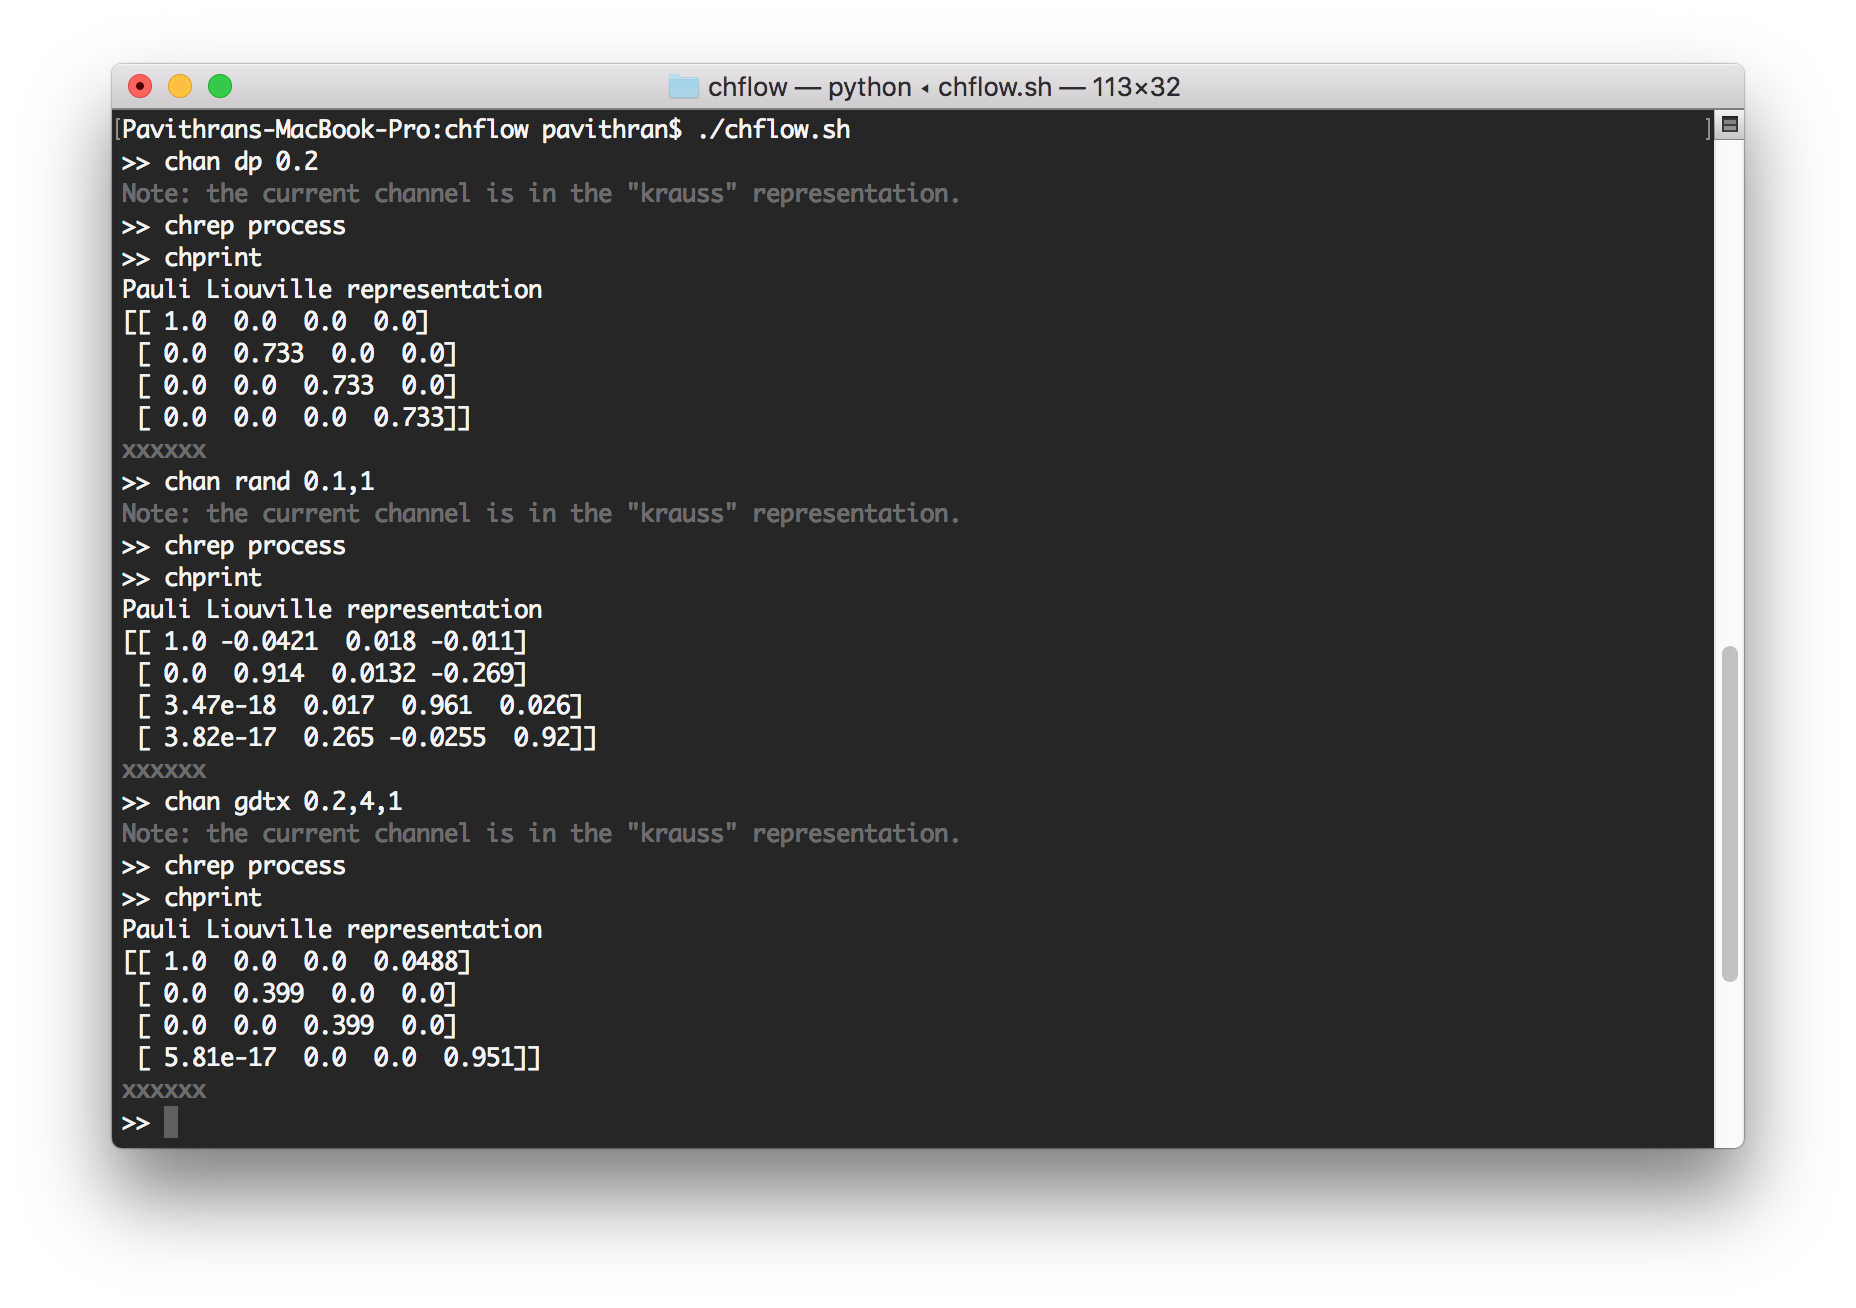
\includegraphics[scale=0.27]{chandefs.jpg}
\caption{The \texttt{chan} command can be used to define quantum channels. For multi-parameter channels, the values of the parameters must be separated by commas.}
\label{fig:predefchans}
\end{center}
\end{figure}

\section{Defining you own quantum channels}
In addition to the predefined channels in table \ref{predefchans}, one can also define a quantum channel in two distinct ways. First, by supplying the explicit form of the quantum channel in one of the many representations: Krauss operators, Pauli Liouville matrix, Choi matrix, Chi matrix and Stinespring dilation. The corresponding array form must be stored in a numpy formatted (\texttt{.npy}) or a text file. For eg. \texttt{fname.npy}. This definition can be recalled in \texttt{chflow} as: \texttt{chan fname.npy}.

Second, a symbolic definition of a quantum channel. Here again, one can choose any desired representation, except the Krauss operators, of the underlying quantum channel and provide the corresponding matrix as a text file. The list of variables must be first provided, separated by spaces, with the keyword \texttt{vars}, see fig. \ref{fig:chandef} for example. Some of the entries in the channel description can now be represented by variables and symbolic expressions involving the variables. Mathematical expressions involving symbols must be in a Python interpretable format, since the \hyperlink{pydoceval}{inbuilt command \texttt{eval(...)}} will be under to interpret the expressions.
Finally, the channel definition can be recalled in \texttt{chflow} by providing the file-name as in fig. \ref{fig:predefchans}, followed by the values of the variables separated by commas (if necessary). We will illustrate the definition using an example of a stochastic quantum channel that performs the Clifford operations $H$ and $S$ with equal probabilities, $p/2$ for some $p\in[0,1]$. This channel has the following Krauss representation:
\begin{gather}
\cE(\rho) = (1 - p - q)\thickspace \rho + p\thickspace H\rho H + q\thickspace S\rho S
\end{gather}
and the Pauli Liouville matrix
\begin{gather}
\Gamma =
\begin{pmatrix}
1 & 0 & 0 & 0 \\
0 & 1-p-q & p & q \\
0 & -p & 1-p-2q & 0 \\
0 & q & 0 & 1-q
\end{pmatrix} . \label{eq:filechan}
\end{gather}
To specify the channel using its Pauli Liouville matrix $\Gamma$, we must create a text file with the description of $\Gamma$, as shown in the figure below.
\begin{figure}[H]
\begin{center}
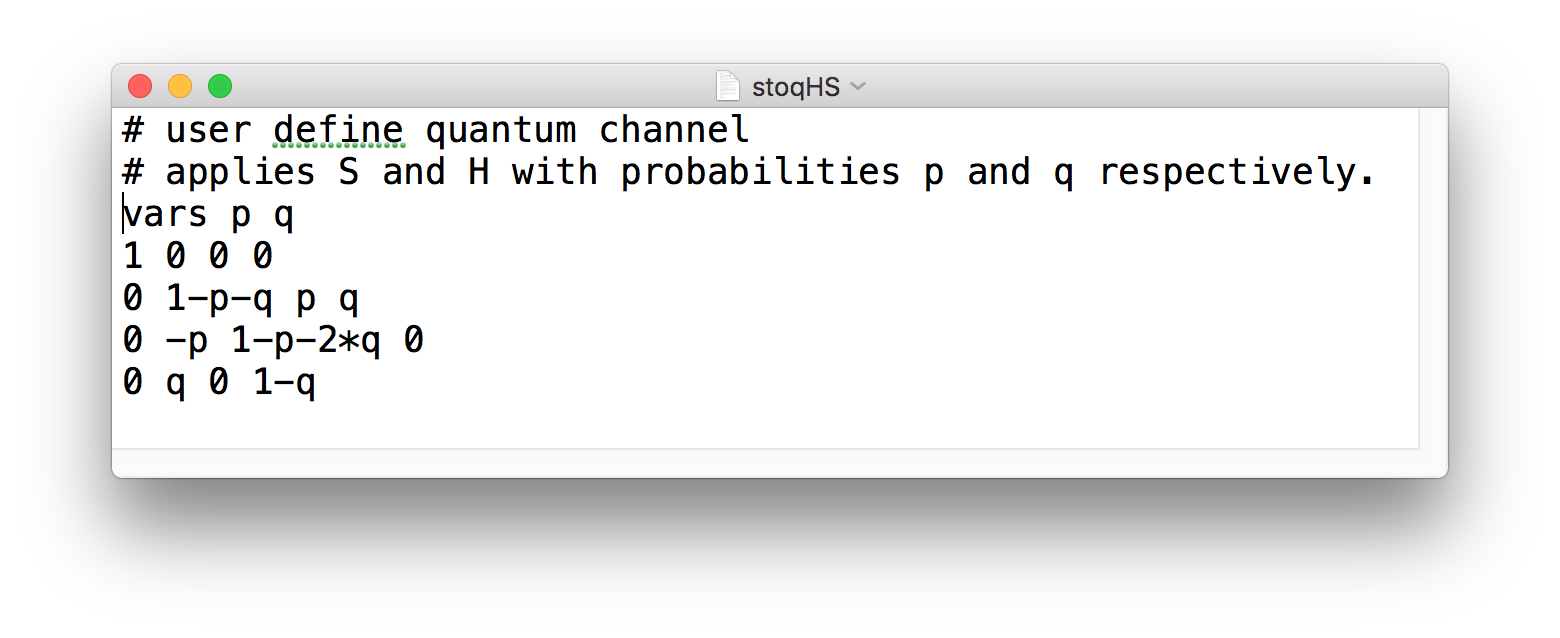
\includegraphics[scale=0.25]{filechandef.jpg}
\caption{Description of $\Gamma$ as mentioned in eq. \ref{eq:filechan} in a text file. The above file can be found in \href{run ./../examples/stoqHS.txt}{\texttt{examples/stoqHS.txt}}.}
\label{fig:chandef}
\end{center}
\end{figure}
Note that the order of variables in \texttt{vars} must be the same as the order of parameter values, provided while recalling the channel definition using \texttt{chan} (see fig. \ref{predefchans}). Lines commencing with ``\#'' are only for commenting purposes, they will be ignored by \texttt{chflow}.
\section{References}
\begin{enumerate}
\item \hypertarget{pydoceval}{\url{https://docs.python.org/2/library/functions.html\#eval}}.
\end{enumerate}
\end{document}